\documentclass{beamer}
\usepackage[utf8]{inputenc}
\usepackage{threeparttable}
%\usepackage{utopia} %font utopia imported
\usepackage{amsthm, booktabs, setspace, natbib, amsfonts,amssymb,epstopdf,textcomp,listings, xcolor}

\usepackage{adjustbox} % Shrink stuff
\usepackage{pgfpages}


\usepackage{tikz}
\usepackage{verbatim}
\setbeamertemplate{note page}{\pagecolor{yellow!5}\insertnote}
\usetikzlibrary{positioning}
\usetikzlibrary{snakes}
\usetikzlibrary{calc}
\usetikzlibrary{arrows}
\usetikzlibrary{decorations.markings}
\usetikzlibrary{shapes.misc}
\usetikzlibrary{matrix,shapes,arrows,fit,tikzmark}

\usepackage{amsmath}
\usepackage{mathpazo}
\usepackage{hyperref}
\usepackage{lipsum}
\usepackage{multimedia}
\usepackage{graphicx}
\usepackage{multirow}
\usepackage{dcolumn}
\usepackage{bbm}
\usepackage[space]{grffile}
\usepackage{tabularx}
\usepackage{subfig}
\usepackage{float}
\usepackage{multirow}

\usepackage{tabularx}
\usepackage{fancyhdr}
\usepackage{lscape}
\usepackage{mdframed}
\usepackage{mathtools}
\usepackage{array}

\usepackage{mwe}
\usepackage[skip=2pt,font=scriptsize]{caption}
\captionsetup{labelfont=bf, format=hang, labelsep=period, labelformat = empty}
%labelformat  =simple
%labelformat = empty

\usepackage{appendixnumberbeamer} %for avoid counting appendix slides add \appendix
\usepackage{colortbl}
\usepackage{xcolor}

%\usetheme{Warsaw}
\usetheme{Madrid}
\usecolortheme{default}
\usepackage{natbib}
\bibliographystyle{unsrtnat}


%------------------------------------------------------------
%This block of code defines the information to appear in the
%Title page
\title[Genetic Dilution in Improved Maize] %optional/
{A Case of Genetic Dilution in Improved Maize: Estimating
Comparative Advantage of Adoption in Ethiopia}


\author[]{Aleksandr Michuda\inst{1} \and Cristina Chiarella\inst{2} \and Oscar Barriga-Cabanillas\inst{3} \and Juan Correa\inst{4}}

\institute[]{\inst{1} Cornell University \and \inst{2} UCLouvain \and \inst{3} World Bank Corp. \and \inst{4} FAO}

% \institute[UC Davis] % (optional)
% {
% %  \inst{1}%
%   Agricultural and Resource Economics\\
%   UC Davis
%  }

\date[November 2022] % (optional)
{NEUDC   \\
November 2022}


%End of title page configuration block
%------------------------------------------------------------



%------------------------------------------------------------
%The next block of commands puts the table of contents at the 
%beginning of each section and highlights the current section:

\AtBeginSection[]
{
  \begin{frame}
    \frametitle{Table of Contents}
    \tableofcontents[currentsection]
  \end{frame}
}
%------------------------------------------------------------


\begin{document}

\setbeamertemplate{enumerate items}[square]
\setbeamercolor{item projected}{bg=none,fg=black}

%\setbeamercolor{enumerate items}{〈key=value〉 list} to
%\setbeamercolor{item projected}{bg=none,fg=beamer@blendedblue}

\setbeamertemplate{itemize items}[circle]
\setbeamercolor{itemize item}{fg=black}
\setbeamercolor{itemize subitem}{fg=black}

%%% TIKZ STUFF
\tikzset{   
        every picture/.style={remember picture,baseline},
        every node/.style={anchor=base,align=center,outer sep=1.5pt},
        every path/.style={thick},
        }
\newcommand\marktopleft[1]{%
    \tikz[overlay,remember picture] 
        \node (marker-#1-a) at (-.3em,.3em) {};%
}
\newcommand\markbottomright[2]{%
    \tikz[overlay,remember picture] 
        \node (marker-#1-b) at (0em,0em) {};%
}
\tikzstyle{every picture}+=[remember picture] 
\tikzstyle{mybox} =[draw=black, very thick, rectangle, inner sep=10pt, inner ysep=20pt]
\tikzstyle{fancytitle} =[draw=black,fill=red, text=white]
%%%% END TIKZ STUFF



%The next statement creates the title page.
\frame{\titlepage}

% %---------------------------------------------------------
% %This block of code is for the table of contents after
% %the title page
% \begin{frame}
% \frametitle{Table of Contents}
% \tableofcontents
% \end{frame}
% %---------------------------------------------------------




%---------------------------------------------------------
\begin{frame}
\frametitle{Introduction}

Food security is a major challenge: Ethiopia is no exception

\begin{itemize}
    % \item Struggled to provide an adequate and reliable food supply
    \item Breakthroughs in maize germplasm ($\uparrow$ yields, $\uparrow$ drought tolerance)
\end{itemize}

However adoption of improved seed has remained a challenge:

\begin{enumerate}[ {[}1{]} ]
    \item Lack of market integration \citep{Carter2014-fm, adejobi2013markets}
    \item Access to supplementary inputs \citep{Byerlee2013-qk, Munshi2004-og}
    \item Adaptation to agro-ecological conditions \citep{Bird2020-nt}
    \item Tech. Transfer Challenges of learning \citep{Conley2010-ue}
\end{enumerate}

\end{frame}

\begin{frame}{Research Question}

\textbf{How does misclassification in adoption status mask heterogeneous impacts to adoption?}
\end{frame}

\begin{frame}{Preview of Results}

\begin{enumerate}[ {[}1{]} ]
    \item Explore heterogeneous comparative advantages through GRrC (reformulation of \cite{Suri2011-oi}): find puzzling results.
    \item Endogenous switching regression with different definitions of improved seeds: self-reported, second generation or recycled, purity of genetic material, year of release, types and source.
    \item Low adoption of newest and purest varieties, which \textit{in fact} return higher yields. 
    \item Due to genetic dilution, all farmers are using improved seed; biasing results
    \item When we account for misclassification in GRrC, the puzzle is resolved
\end{enumerate}
\end{frame}


%---------------------------------------------------------
\begin{frame}
\frametitle{Ethiopian Maize}

\begin{itemize}
    % \item Struggled to provide an adequate and reliable food supply
    \item Use ESS waves 1-4, agricultural questionnaires
    \item Waves 1-3 were a panel and included information on yields, inputs and hybrid maize adoption
    \item Wave 4 is a break from Waves 1-3, but contains similar information $+$ DNA fingerprinting
    \item We focus on maize producing households 
    \item Self-reported use of improved seed varieties and yields
\end{itemize}

\begin{figure}
    \centering
    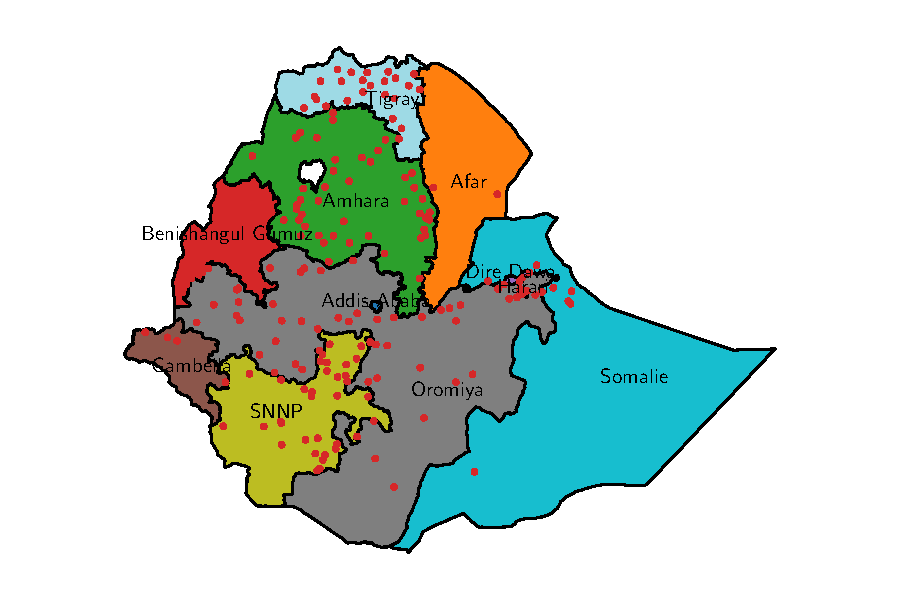
\includegraphics[scale=.4]{results/figures/map_hhids.pdf}
\end{figure}

% \textit{Add interesting image}
\end{frame}

\begin{frame}{}

\begin{figure}
    \centering
    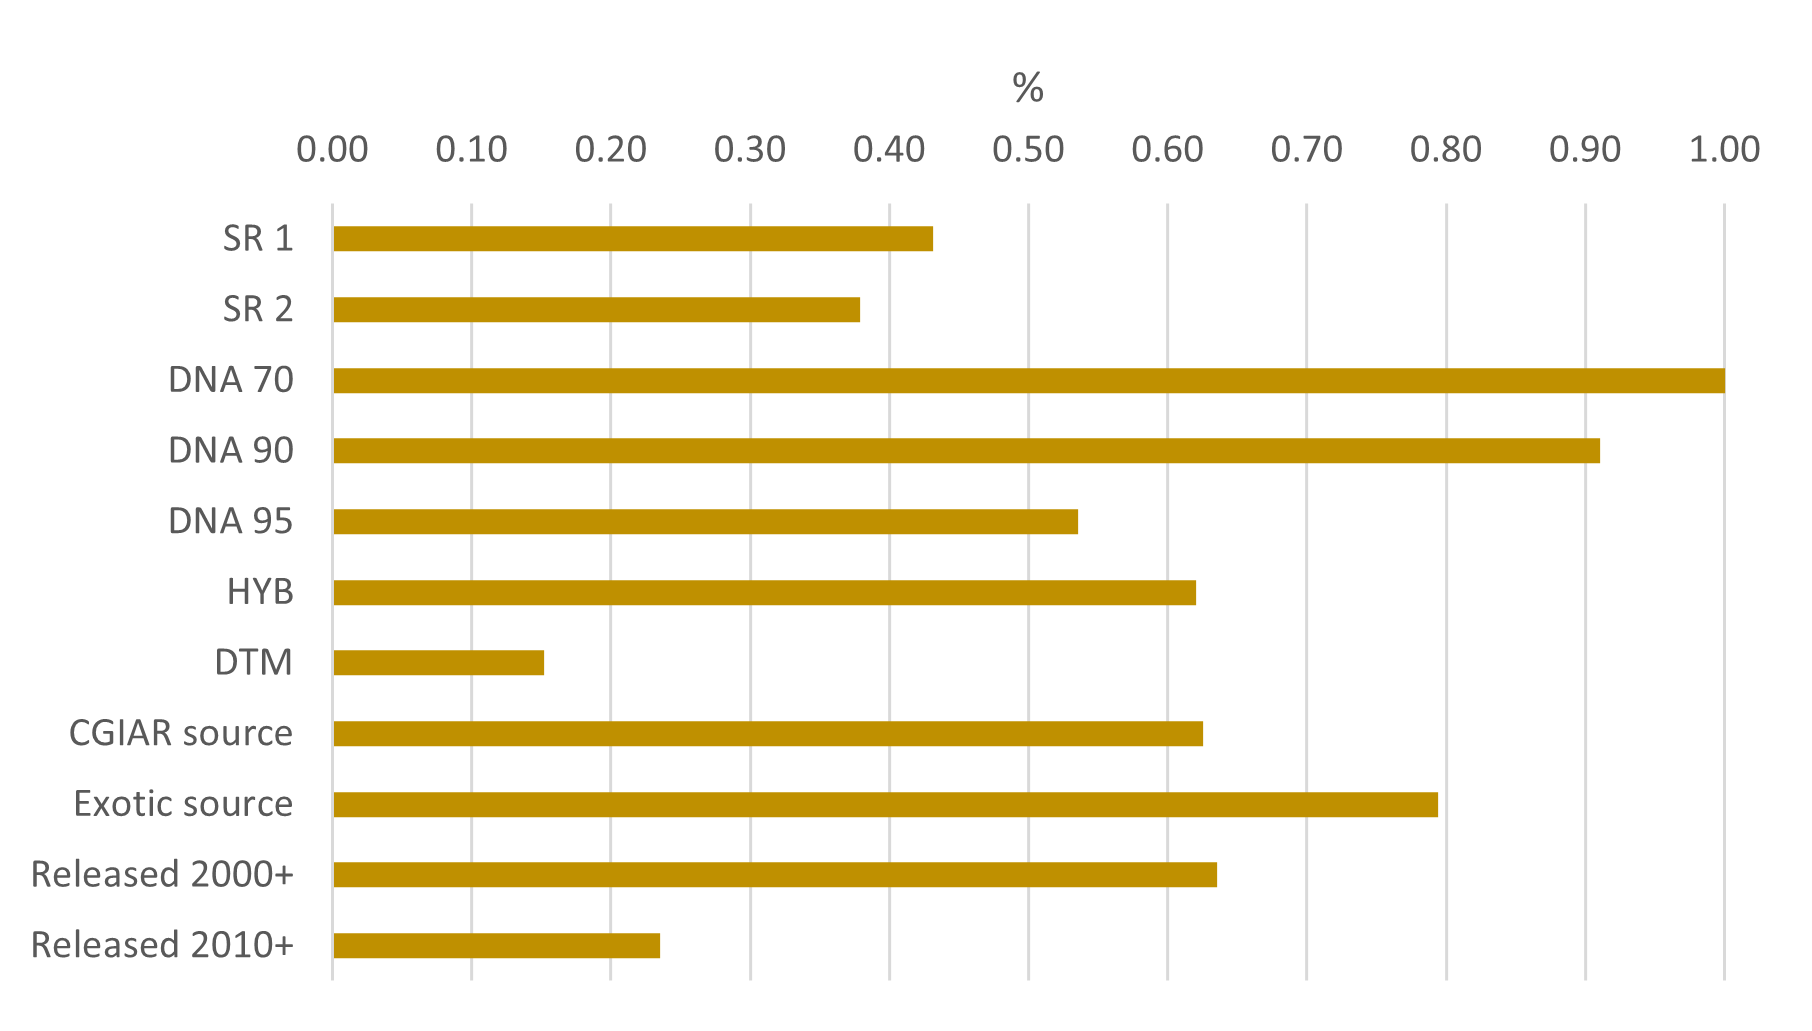
\includegraphics[width=.7\textwidth]{results/figures/adoption_r4.png}
    \caption{Seed varieties: Adoption rate of improved seed varieties in 2018 (by self-report, purity level, crop type, source and year of release)}
\end{figure}
    
\end{frame}

%---------------------------------------------------------
\begin{frame}
\frametitle{Empirical Strategy}

\textbf{Understand the returns of adopting improved varieties: }
\begin{itemize}
    \item Some farmers are ``more suited'' for adoption (comparative advantage) \citep{Suri2011-oi}
    \item How comparative advantage plays a role on using improved seed varieties and its returns.
    \item Use Group Random Coefficient (GrRC) method \citep{Tjernstrom_Emilia_Dalia_Ghanem_Oscar_Barriga_Cabanillas_Travis_J_Lybbert_Jeffrey_D_Michler_and_Aleksandr_Michuda2020-bc} to  separate returns from those who ``should'' be getting highest returns.
\end{itemize}  

% (Suri 2011; Tjernstr\"{o}m et al. 2020; Michler et al. 2019; Barriga et al. 2018)

We estimate a Correlated Random Coefficient Model by way of GrRC estimation:
\vspace{-2em}
\begin{center}
$$
    y_{it}= \delta + \Delta h_{it} + \phi\boldsymbol{\theta_i} h_{it} + \tau_{i} + \boldsymbol{\theta_i} + \epsilon_{it}
$$  
\end{center}

\end{frame}


%---------------------------------------------------------
\begin{frame}
\frametitle{Empirical Strategy}
\begin{enumerate}
    \item Identification does not require IV
    \item Identification similar to \cite{Chamberlain1984-uk}: strict exogeneity
    \item Strong assumption, but gives us ability to estimate returns to adoption, as well as \textit{advantage in adopting}
    \item Requires enough variation in ``switcher trajectories'' 
\end{enumerate}
\end{frame}

\begin{frame}{Trajectories}
\begin{table}
\centering
\caption{Trajectories of Households}
\label{tbl:trajectories}
\begin{tabular}{lrr}
\toprule
Trajectory &  Frequency &    Share \\
\midrule
       000 &       2124 & 0.611927 \\
       111 &        456 & 0.131374 \\
       011 &        228 & 0.065687 \\
       001 &        219 & 0.063094 \\
       010 &        153 & 0.044080 \\
       100 &        108 & 0.031115 \\
       110 &         96 & 0.027658 \\
       101 &         87 & 0.025065 \\
\bottomrule
\multicolumn{3}{l}{Note: Table shows frequency and shares of each trajectory in sample. 1 denotes adoption and 0 otherwise. The first digit is for whether the household adopted in wave 1, the second digit for wave and the third digit for wave 3}
\end{tabular}
\end{table}


\end{frame}


%---------------------------------------------------------
%---------------------------------------------------------
\begin{frame}
\frametitle{The Puzzle: Using high yield varieties does not improved returns}
% \frametitle{Group Random Coefficients Results}

\begin{figure}
    \centering
    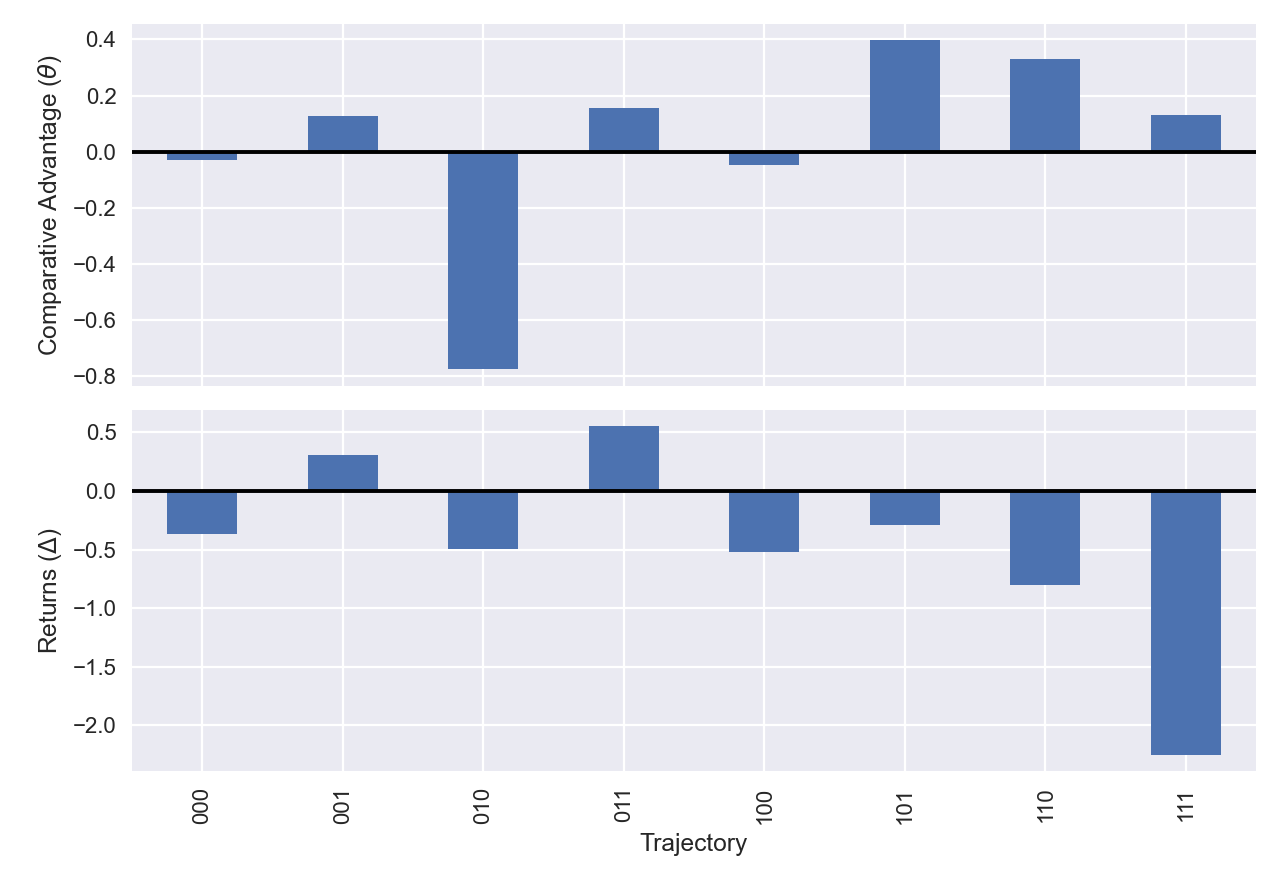
\includegraphics[scale=0.5]{results/figures/theta.png}\label{fig:theta_delta_raw}
\end{figure}
 
\end{frame}

%---------------------------------------------------------

%---------------------------------------------------------
\begin{frame}
\frametitle{What's going on?}

\begin{itemize}
    \item Negative advantage to adopting
    \item Adopting more associated with less advantage
    \item Negative returns (but that's part of the standard story about access)
\end{itemize}

\end{frame}

\begin{frame}{How do we resolve this puzzle?}
\begin{itemize}
    \item Use the  4th wave of the survey to leverage DNA-fingerprinting information 
    \item DNA allows us to assess what varieties (and purity) farmers are in reality planting  
    \item We implement an endogenous switching regression approach to properly measure yield return 
    \item Assess the genetic purity of improved varieties, year of release, types and sources
\end{itemize}


\end{frame}
%---------------------------------------------------------


%---------------------------------------------------------
\begin{frame}
\frametitle{Endogenous Switching Regression Results}

\begin{table}[H]
\resizebox{.75\textwidth}{!}{
\centering
\hspace*{-1.2cm}
\begin{threeparttable}
\caption{Effects on yields (log) from adopting improved maize varieties (DNA fingerprinting)}
\label{tab:switch2}
\begin{tabular}{l cccccc}
\hline
\hline
            &Adopters yields&Non-adopters yields&         ATE&          SE&     p-value\\
\hline
\textit{DNA 70, SR yields}&            &            &            &            &            \\
ATT         &        7.17&        7.31&      \fcolorbox{red}{lightgray}{-0.14}&       0.026&      0.0000\\
%
%
%
ATU         &        8.76&        6.76&        2.00&       0.036&      0.0000\\
%
%
%
\textit{DNA 90, SR yields}&            &            &            &            &            \\
ATT         &        7.18&        9.07&       \fcolorbox{red}{lightgray}{-1.90}&       0.023&      0.0000\\
%
%
%
ATU         &        7.01&        6.80&        0.21&       0.022&      0.0000\\
%
%
%
\textit{DNA 95, SR yields}&            &            &            &            &            \\
ATT         &        7.30&        7.08&        \fcolorbox{red}{lightgray}{0.22}&       0.036&      0.0000\\
%
%
%
ATU         &        6.87&        6.86&       0.018&       0.029&      0.5496\\
%
%
%
\textit{HYB, SR yields}&            &            &            &            &            \\
ATT         &        7.28&        7.25&       \fcolorbox{red}{lightgray}{0.030}&       0.028&      0.2892\\
%
%
%
ATU         &        7.06&        6.85&        0.21&       0.028&      0.0000\\
%
%
%
\textit{DTMZ, SR yields}&            &            &            &            &            \\
ATT         &        7.42&        6.53&        \fcolorbox{red}{lightgray}{0.89}&       0.074&      0.0000\\
%
%
%
ATU         &        7.11&        7.02&       0.089&       0.022&      0.0001\\
%
%
%
\textit{CGIAR source, SR yields}&            &            &            &            &            \\
ATT         &        7.13&        6.71&        \fcolorbox{red}{lightgray}{0.43}&       0.033&      0.0000\\
%
%
%
ATU         &        9.19&        6.89&        2.31&       0.018&      0.0000\\
%
%
%
\textit{Year 2010+, SR yields}&            &            &            &            &            \\
ATT         &        7.44&        6.92&        \fcolorbox{red}{lightgray}{0.53}&       0.039&      0.0000\\
%
%
%
ATU         &        8.98&        6.91&        2.07&       0.056&      0.0000\\
%
%
%
\hline
\hline
\end{tabular}
\end{threeparttable}
}
\end{table}
 
\end{frame}
%---------------------------------------------------------

%---------------------------------------------------------
\begin{frame}
\frametitle{Discussion}
Negative and small returns to adoption from self-reported improved varieties.
\begin{itemize}
    \item But positive returns to more genetically pure, DTMZ, CG- sourced and newer varieties.
    \item All DNA fingerprints are 70\% pure or higher. Control group has high share of false positives: no proper  control.  
\end{itemize}

Could misclassification be masking returns heterogeneity?
\begin{itemize}
    \item If farmers using genetically diluted hybrid, or older generations, this would attenuate effects
    \item Trajectories would be misclassified.
\end{itemize}

\end{frame}

\begin{frame}{Misclassification Driving Returns?}
\begin{itemize}
    \item We estimate a misclassification robust GRrC 
    \item A Maximum likelihood estimation approach uses misclassification rates to properly estimate coefficients on the returns from adoption of high yield varieties $-$inspired by \cite{michuda2021three}
    \item We apply wave 4 misclassification rates for waves 1-3
\end{itemize}

\begin{equation*}
\label{eq:mr-GRrC}
l(\mu, \kappa, \Delta, \beta, \sigma|y_{t}, \hat{h}) = \sum_{\underbar{$h$}\in\mathcal{H}} \left[ f_{Y_{t}| \mathcal{H}}(y|h=\underbar{$h$})\cdot  \sum_{\bar{h} \in \mathcal{H}} \boldsymbol{1\{\hat{h}=\bar{h}\} p_{\underbar{$h$}, \bar{h}}} \right]
\end{equation*}

\end{frame}

\begin{frame}{Misclassification Rates from Wave 4}

\begin{itemize}
    \item Use rate of hybrid of at least 95\% purity, against self-reported hybrid use to calculate misclassification
    \item A farmer who reports using traditional seed is actually using hybrid 14\% of the time
    \item A farmer who reports using hybrid seed is actually using traditional seed almost \textit{30\%} of the time.
\end{itemize}
    \begin{table}[]
        \centering
        \begin{tabular}{lll}
        \toprule
         & 0 & 1 \\
        \midrule
        0 & 0.863 & 0.137 \\
        1 & 0.296 & 0.704 \\
        \bottomrule
        \end{tabular}
        \caption{Misclassification Matrix of 95\% genetic purity}
    \end{table}
    
\begin{equation}
    \label{eq:misclass}
    P(h = (i,j,k) , \hat{h} = (\hat{i},\hat{j}, \hat{k})) = p_{i, \hat{i}}\cdot p_{j, \hat{j}}\cdot p_{k, \hat{k}}
\end{equation}
\end{frame}




\begin{frame}{Misclassified GRrC Results}

\begin{figure}
    \centering
    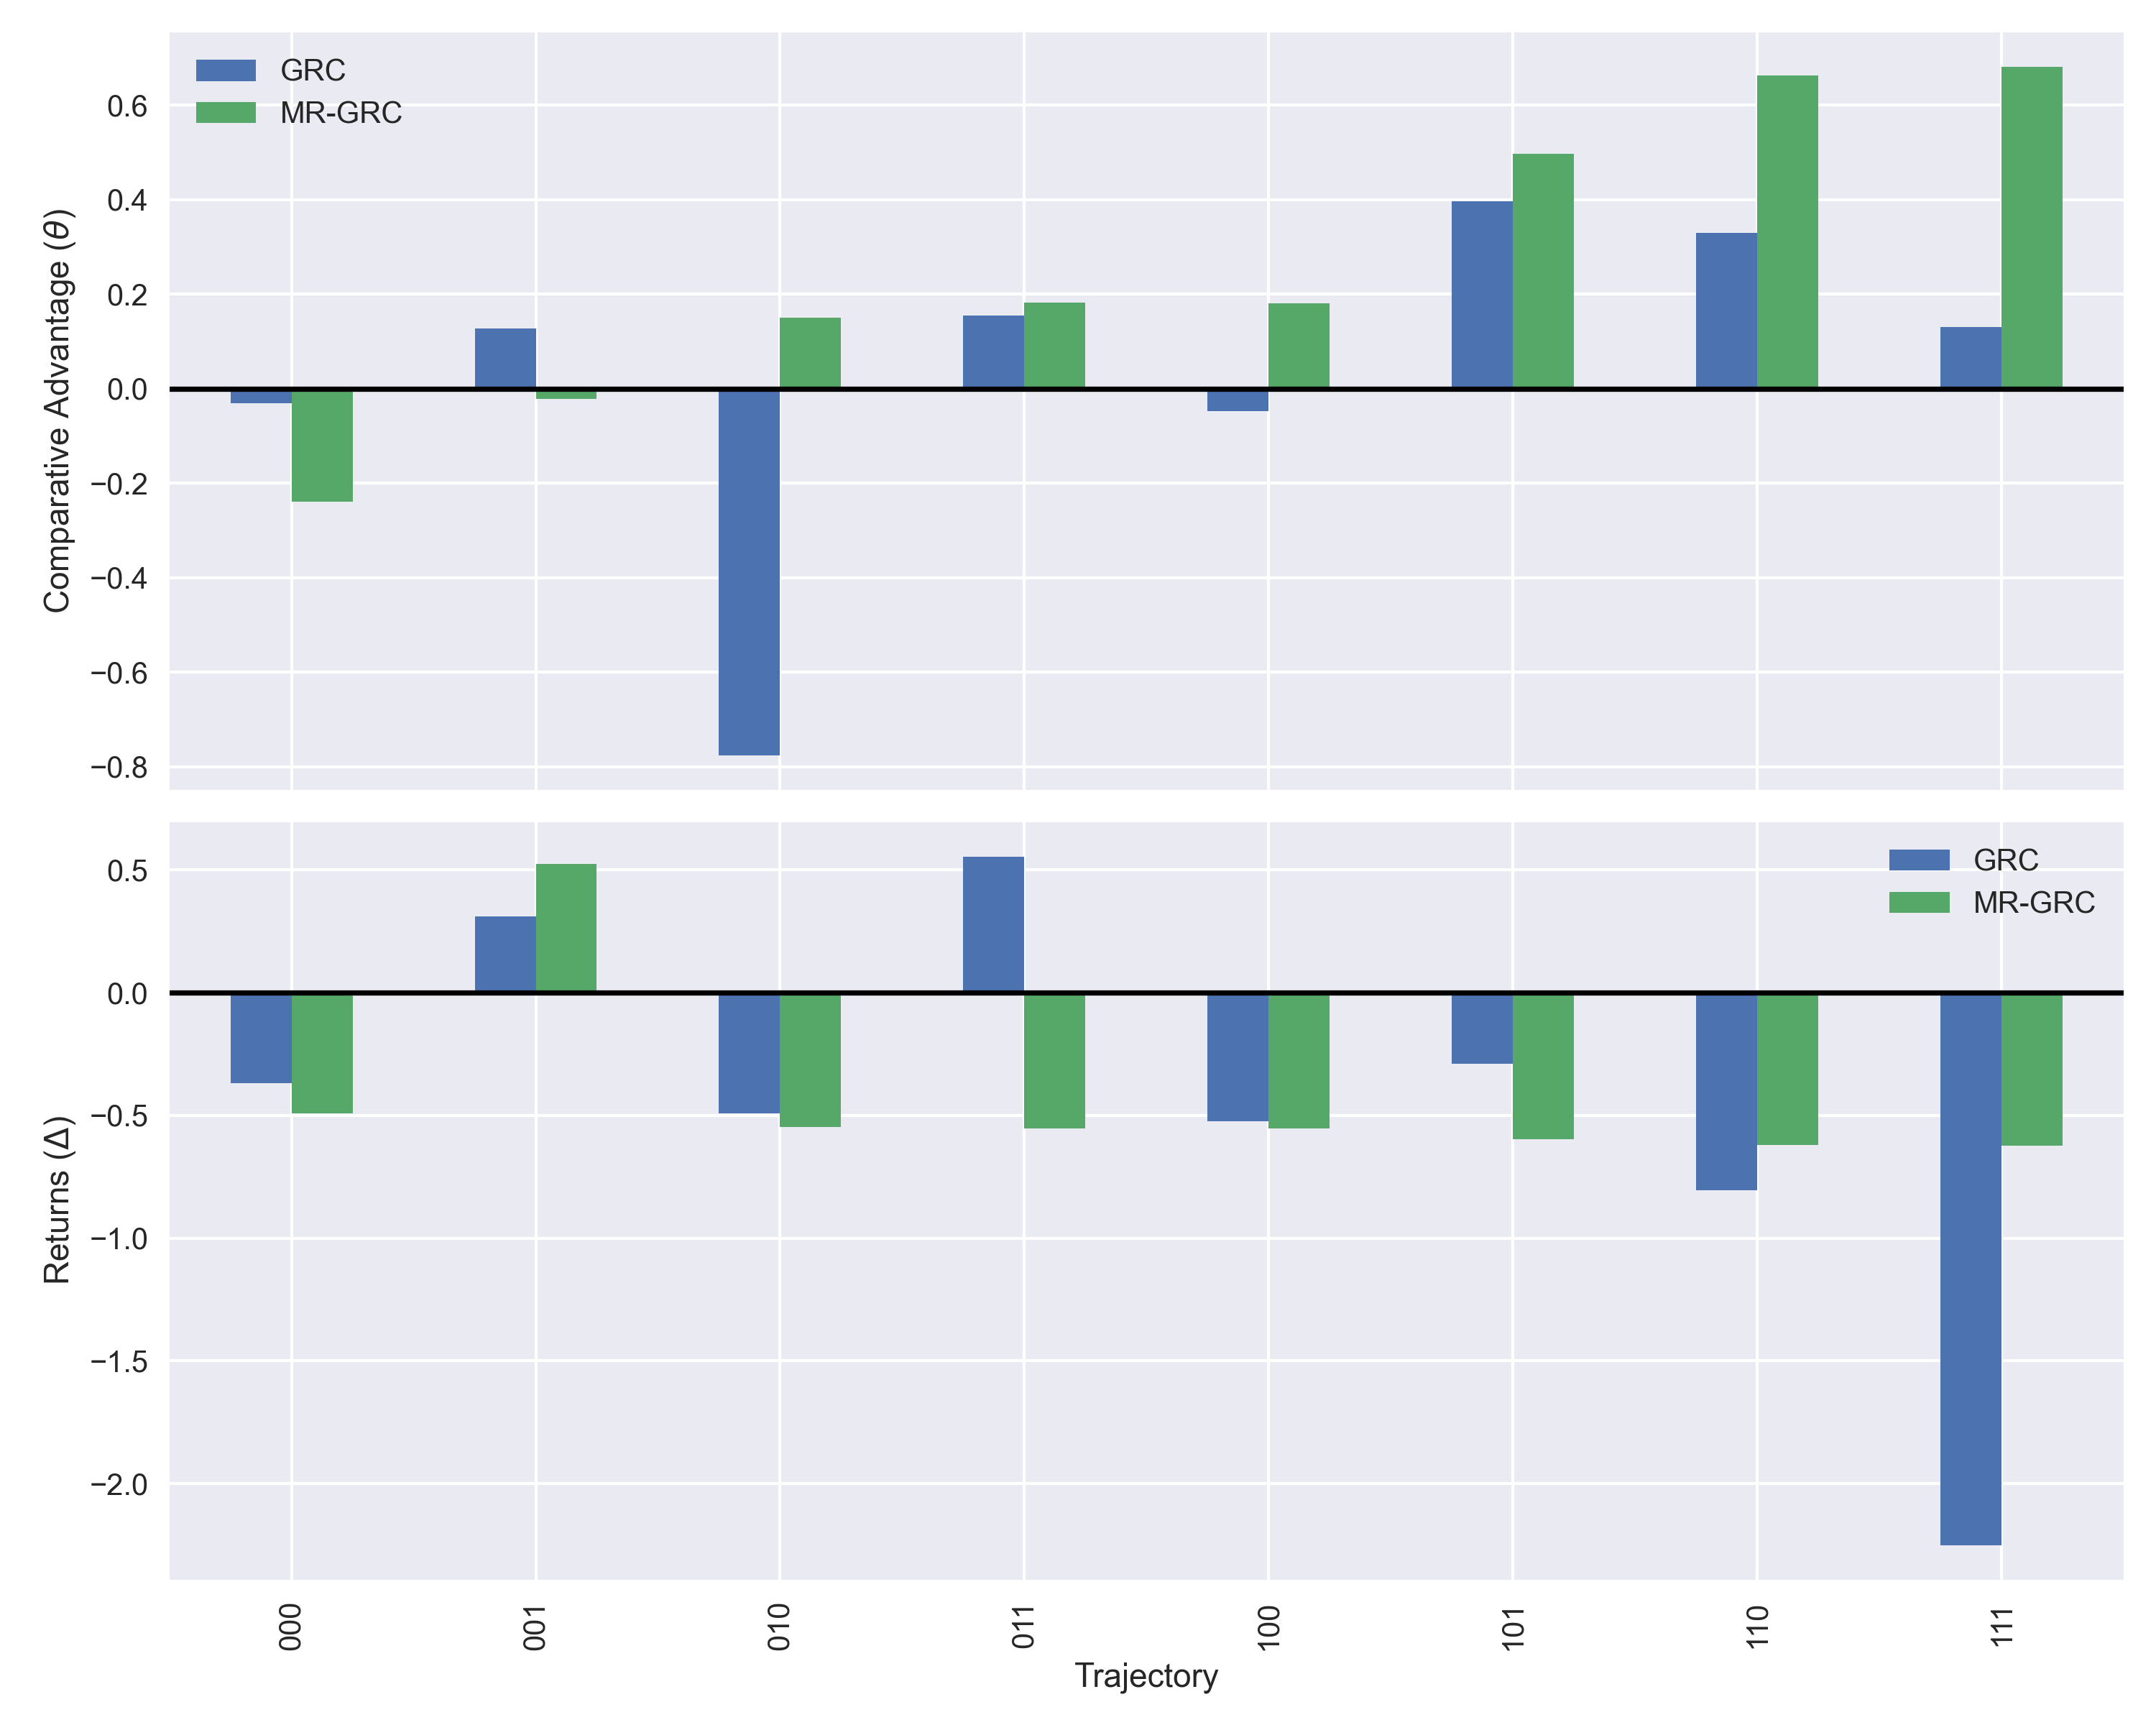
\includegraphics[scale=0.4]{results/figures/mr-theta.png}
\end{figure}
\end{frame}

\begin{frame}{Conclusion}

Accounting for misclassification resolves the issue and makes the adoption problem the classic story about access and a lack of profitability.

\begin{itemize}
    \item Farmers think they're adopting improved seed varieties but evidence shows considerable dilution and varieties are not yielding as expected
    \item Misclassification biases estimates through measurement problem, but also through changes in practices
    \item Mismatch between cultivation practices and seed variety used
    \item Effects of high-yielding varieties diminish over time, but traditional varieties are well adapted to local agro-ecological conditions.
    \begin{itemize}
    \item There may be a threshold in time above which it may be more profitable to use a traditional variety than an improved one that has been around for too many generations.
    \item Example: 010 trajectory
\end{itemize}
\end{itemize}

\end{frame}

\begin{frame}
\textbf{Thank you!}

\begin{itemize}
    \item I would be happy to discuss any questions and please feel free to email me!
    \item am2497@cornell.edu
\end{itemize}


    
\end{frame}

\bibliography{references}

\end{document}